\begin{figure}\centering
	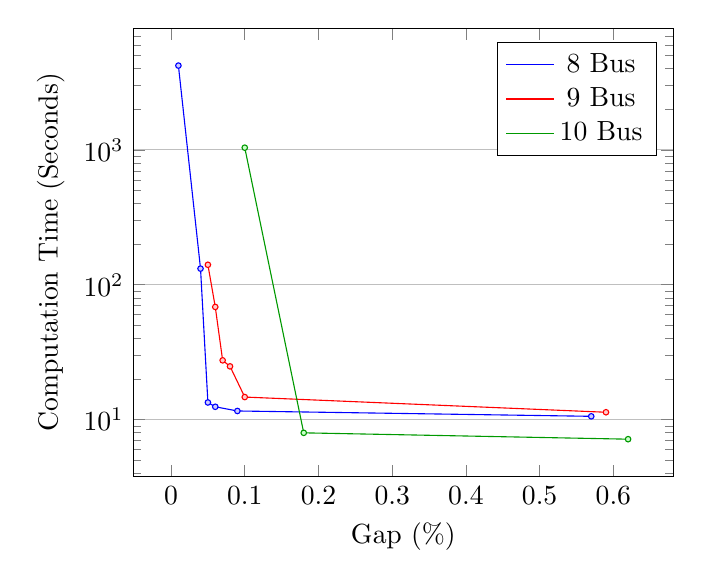
\begin{tikzpicture}
		\begin{axis}[ymajorgrids=true, ylabel={Computation Time (Seconds)}, ymode=log, xlabel={Gap (\%)}, legend pos=north east]%, xtick={0.1, 0.05, 0.01, 0.005, 0.001, 0.0005, 0.0001, 0.00005, 0.00001, 0.000005, 0.000001}, xticklabels={$1\times10^{-1}$, $5\times10^{-2}$, $1\times10^{-2}$, $5\times10^{-3}$, $1\times10^{-3}$, $5\times10^{-4}$, $1\times10^{-4}$, $5\times10^{-5}$, $1\times10^{-5}$, $5\times10^{-6}$, $1\times10^{-6}$}]
			\addplot[blue] coordinates {
				(0.57, 10.58)
				(0.09, 11.59)
				(0.06, 12.45)
				(0.05, 13.40)
				(0.04, 131.78)
				(0.01, 4223.25)
			};
			\addplot[red] coordinates {
				(0.59, 11.34)
				(0.10, 14.70)
				(0.08, 24.83)
				(0.07, 27.51)
				(0.06, 68.49)
				(0.05, 140.70)
			};
			\addplot[green!60!black] coordinates {
				(0.62, 7.16)
				(0.18, 7.98)
				(0.10, 1039.33)
			}; 
			\addplot[fill=blue!20, draw=blue, only marks, mark size=1pt] coordinates {
				(0.57, 10.58)
				(0.09, 11.59)
				(0.06, 12.45)
				(0.05, 13.40)
				(0.04, 131.78)
				(0.01, 4223.25)}; 
			\addplot[fill=red!20, draw=red, only marks, mark size=1pt] coordinates {
				(0.59, 11.34)
				(0.10, 14.70)
				(0.08, 24.83)
				(0.07, 27.51)
				(0.06, 68.49)
				(0.05, 140.70)
			}; 
			\addplot[fill=green!20, draw=green!60!black, only marks, mark size=1pt] coordinates{
				(0.62, 7.16)
				(0.18, 7.98)
				(0.10, 1039.33) 
			};
	\legend{8 Bus, 9 Bus, 10 Bus};
		\end{axis}
	\end{tikzpicture}
	\caption{Comparison of Runtime for a 7-Charger Scenario}
	\label{fig:results:scalabilityTimeVsGap}
\end{figure}


